% Original author of this template:
% Frits Wenneker (http://www.howtotex.com)
\documentclass[paper=letter, fontsize=12pt]{article}
\usepackage[english]{babel} % English language/hyphenation
\usepackage{amsmath,amsfonts,amsthm} % Math packages
\usepackage[utf8]{inputenc}
\usepackage{float}
\usepackage{lipsum} % Package to generate dummy text throughout this template
\usepackage{natbib}
\usepackage{cite}
\usepackage{blindtext}
\usepackage{graphicx} 
\usepackage{caption}
\usepackage{subcaption}
\usepackage[sc]{mathpazo} % Use the Palatino font
\usepackage[T1]{fontenc} % Use 8-bit encoding that has 256 glyphs
\linespread{1.05} % Line spacing - Palatino needs more space between lines
\usepackage{microtype} % Slightly tweak font spacing for aesthetics
\usepackage[hmarginratio=1:1,top=32mm,columnsep=20pt]{geometry} % Document margins
\usepackage{multicol} % Used for the two-column layout of the document
%\usepackage[hang, small,labelfont=bf,up,textfont=it,up]{caption} % Custom captions under/above floats in tables or figures
\usepackage{booktabs} % Horizontal rules in tables
\usepackage{float} % Required for tables and figures in the multi-column environment - they need to be placed in specific locations with the [H] (e.g. \begin{table}[H])
\usepackage{hyperref} % For hyperlinks in the PDF
\usepackage{lettrine} % The lettrine is the first enlarged letter at the beginning of the text
\usepackage{paralist} % Used for the compactitem environment which makes bullet points with less space between them
\usepackage{abstract} % Allows abstract customization
\renewcommand{\abstractnamefont}{\normalfont\bfseries} % Set the "Abstract" text to bold
\renewcommand{\abstracttextfont}{\normalfont\small\itshape} % Set the abstract itself to small italic text
\usepackage{titlesec} % Allows customization of titles

\renewcommand\thesection{\Roman{section}} % Roman numerals for the sections
\renewcommand\thesubsection{\Roman{subsection}} % Roman numerals for subsections
\hypersetup{
    colorlinks,
    citecolor=black,
    filecolor=black,
    linkcolor=black,
    urlcolor=black
}
\newtheorem*{assumption*}{\assumptionnumber}
\providecommand{\assumptionnumber}{}
\makeatletter
\newenvironment{assumption}[2]
 {%
  \renewcommand{\assumptionnumber}{Assumption #1-$\mathcal{#2}$}%
  \begin{assumption*}%
  \protected@edef\@currentlabel{#1-$\mathcal{#2}$}%
 }
 {%
  \end{assumption*}
 }
\makeatother
\setcounter{secnumdepth}{4}

\titleformat{\paragraph}
{\normalfont\normalsize\bfseries}{\theparagraph}{1em}{}
\titlespacing*{\paragraph}
{0pt}{3.25ex plus 1ex minus .2ex}{1.5ex plus .2ex}
\titleformat{\section}[block]{\large\scshape\centering}{\thesection.}{1em}{} % Change the look of the section titles
\titleformat{\subsection}[block]{\large}{\thesubsection.}{1em}{} % Change the look of the section titles
\newcommand{\horrule}[1]{\rule{\linewidth}{#1}} % Create horizontal rule command with 1 argument of height
\usepackage{fancyhdr} % Headers and footers
\pagestyle{fancy} % All pages have headers and footers
\fancyhead{} % Blank out the default header
\fancyfoot{} % Blank out the default footer
\graphicspath{ {./images/} }
\usepackage{enumitem}
\fancyhead[C]{Royal Institute of Technology (KTH) Stockholm $\bullet$ 21 December 2016 $\bullet$ Group 20 } % Custom header text

\fancyfoot[RO,LE]{\thepage} % Custom footer text
%----------------------------------------------------------------------------------------
%       TITLE SECTION
%----------------------------------------------------------------------------------------
\title{\vspace{-15mm}\fontsize{24pt}{10pt}\selectfont\textbf{Distributed Artificial Intelligence and Intelligent Agents (ID2209): Project assignment}} % Article title
\author{
\large
{\textsc{Kim Hammar, Stockholm 16446 }}\\[2mm]
%\thanks{A thank you or further information}\\ % Your name
\normalsize \href{mailto:kimham@kth.se}{kimham@kth.se}\\[2mm] % Your email address
}
\date{}
\begin{document}
\maketitle % Insert title
\thispagestyle{fancy} % All pages have headers and footers


\section{Introduction}
The requirements statement is essentially just a set of articulated requirements for the system/organization to be designed, for structural reasons the requirements are divided into various related models that use different levels of detail. The system in this context is a SmartMuseum Agent Framework, as of following the GAIA methodology \citep{wooldrigde_jennings} I will from here on frequently use the \textit{organization} metaphor when referring to the system.
\section{Task 1 - Modeling with GAIA Methdology}
\subsection{Analysis}
\subsubsection{Requirements Statement}
\paragraph{Mission Statement}
The SmartMuseum organization has the purpose of connecting different people and entities that are in some sense involved in consuming or providing services related to art. The goal of the organization is to improve the overall experience for everyone involved. The organization should make it easier for consumers to view and find interesting art, for art-curators to provide art and reach out to consumers, for tourguides to find interested consumers as well as building relevant tours and finally for artists to sell their work.

\paragraph{Organization Description}
The activity of a consumer viewing an art-artifact involves atleast three, sometimes four, or five main divisions: \textit{tour-guide division}, \textit{art-curator division}, \textit{artist-management division}, \textit{user-service division} and \textit{artist-division}.
The activity is initiated by the  consumer who contacts the user-service division and selects some type of art-service, the user-service divison support the consumer in requesting/retrieving the service from either the art-curator division or tour-guide-division. In parellel to managing consumer requests the tour-guide division browses art-artifacts that is curated by the art-curator division. Further more, the art-curator divison participates in auctions for obtaining art-artifacts from the artist-management division, in parallel to managing requests from consumers and tourguides. Finally, the artist-management division initiates auctions for art-artifacts on request from artists.

The activities described above can the be modelled as an organization in the following way. The organization consists of $7$ roles. The \textsc{ArtConsumer (AC)} who consumes arts in different forms. The \textsc{UserHandler (UH)} which the consumer uses to purchase and browse services related to art. The \textsc{TourGuide (TA)} which builds and offers virtual tours. The \textsc{ArtBuyer (AB)} who buys art to include in its gallery/museum, the \textsc{ArtQuoter (AQ)} who quotes the price for arts and sells it to consumers. The \textsc{ArtSeller (AS)} who sells art-artifacts produced by artists. And finally the \textsc{Artist (A)} who produces art.
\subsubsection{Roles Model}
\begin{assumption}{1}{A}\label{1A}
Roles can find each other in some way in order to communicate
\end{assumption}
\begin{figure}[H]
  \begin{center}
\noindent\fbox{%
    \parbox{\textwidth}{%
\setlength\parindent{14pt} Role Schema: \hspace{1em} \textsc{ArtConsumer (AC)}\\
\setlength\parindent{14pt} \noindent\rule{15cm}{0.4pt}

\setlength\parindent{14pt} Description: 
\par\setlength\parindent{44pt} Initiates activity of consuming art, which includes purchasing some service \\
\setlength\parindent{14pt} \noindent\rule{15cm}{0.4pt}

\setlength\parindent{14pt} Protocols and activities: 
\par\setlength\parindent{44pt} {\fontfamily{\sfdefault}\selectfont 
DownloadVirtualTour, BuyArt, \underline{ConsumeService}
} \\
\setlength\parindent{14pt} \noindent\rule{15cm}{0.4pt}

\setlength\parindent{14pt} Permissions: 
\par\setlength\parindent{104pt}$\text{\textbf{reads}}$ \hspace{2.8em} $\text{{\fontfamily{\sfdefault}\selectfont supplied }}availableServices \quad \text{\textit{//}} \quad \text{\textit{list of services}}$
\par\setlength\parindent{162pt}$money$\hspace{8.9em} $\text{\textit{//}} \quad \text{\textit{money of the consumer}}$
\par\setlength\parindent{104pt}$\text{\textbf{generates}}$ \hspace{0.9em} $valuation$\hspace{7.5em} $\text{\textit{//}} \quad \text{\textit{valuation of selected artifact}}$
\par\setlength\parindent{162pt}$artifactTitle$\hspace{6.1em} $\text{\textit{//}} \quad \text{\textit{title of selected artifact}}$\
\par\setlength\parindent{162pt}$virtualTourTitle$\hspace{4.4em} $\text{\textit{//}} \quad \text{\textit{title of selected virtual-tour}}$\
\par\setlength\parindent{162pt}$virtualTourTitle$\hspace{4.4em} $\text{\textit{//}} \quad \text{\textit{valuation of selected virtualTour}}$
\par\setlength\parindent{162pt}$moneyForArtifact$\hspace{3.4em} $\text{\textit{//}} \quad \text{\textit{money for selected artifact}}$\\
\setlength\parindent{14pt} \noindent\rule{15cm}{0.4pt}

\setlength\parindent{14pt} Responsibilities
\par \setlength\parindent{14pt} Liveness:
\par\setlength\parindent{75pt}$\text{\textsc{ArtConsumer}} = (\text{{\fontfamily{\sfdefault}\selectfont 
GetService. \underline{ConsumeService}
}})^{\omega}$
\par\setlength\parindent{75pt}$\text{\textsc{GetService}} = (\text{{\fontfamily{\sfdefault}\selectfont 
DownloadVirtualTour |  BuyArt}})$

\par \setlength\parindent{14pt} Safety:
\begin{itemize}[leftmargin=20mm]
\item \textbf{true}
\end{itemize}
    }%
}
\caption{Schema for role \textsc{ArtConsumer}}
\label{fig:role_art_consumer}
\end{center}
\end{figure}

\begin{figure}[H]
  \begin{center}
\noindent\fbox{%
    \parbox{\textwidth}{%
\setlength\parindent{14pt} Role Schema: \hspace{1em} \textsc{UserHandler (UH)}\\
\setlength\parindent{14pt} \noindent\rule{15cm}{0.4pt}

\setlength\parindent{14pt} Description: 
\par\setlength\parindent{44pt} Receives request to buy art-services from consumers and manages the process of the \par\setlength\parindent{44pt}consumer purchasing and obtaining the service. \\
\setlength\parindent{14pt} \noindent\rule{15cm}{0.4pt}

\setlength\parindent{14pt} Protocols and activities: 
\par\setlength\parindent{44pt} {\fontfamily{\sfdefault}\selectfont 
ManageArtPayment, GetVirtualTour, GetArtifactsList,
} 
\par\setlength\parindent{44pt} {\fontfamily{\sfdefault}\selectfont GetVirtualTourList, \underline{GenerateListOfArtServices}}\\
\setlength\parindent{14pt} \noindent\rule{15cm}{0.4pt}

\setlength\parindent{14pt} Permissions: 
\par\setlength\parindent{84pt}$\text{\textbf{generates}}$ \hspace{1em} $ availableServices \quad $ \hspace{3.6em} $\text{\textit{//}} \quad \text{\textit{list of services}}$
\par\setlength\parindent{143pt}$bid \quad $ \hspace{9.6em} $\text{\textit{//}} \quad \text{\textit{bid to attempt to buy artifact}}$
\par\setlength\parindent{84pt}$\text{\textbf{reads}}$ \hspace{2.9em} $ \text{{\fontfamily{\sfdefault}\selectfont supplied }}virtualTours$ \hspace{2.8em} $\text{\textit{//}} \quad \text{\textit{list of virtual tours}}$
\par\setlength\parindent{143pt}$\text{{\fontfamily{\sfdefault}\selectfont supplied }}artifacts $ \hspace{4.5em}$\text{\textit{//}} \quad \text{\textit{list of art-artifacts}}$
\par\setlength\parindent{143pt}$\text{{\fontfamily{\sfdefault}\selectfont supplied }}money$\hspace{5.5em} $\text{\textit{//}} \quad \text{\textit{money of the consumer}}$
\par\setlength\parindent{143pt}$\text{{\fontfamily{\sfdefault}\selectfont supplied }}artifactTitle$\hspace{2.9em} $\text{\textit{//}} \quad \text{\textit{title of artifact-purchase}}$
\par\setlength\parindent{143pt}$\text{{\fontfamily{\sfdefault}\selectfont supplied }}virtualTourTitle$\hspace{1.1em} $\text{\textit{//}} \quad \text{\textit{title of virtual-tour selection}}$
\par\setlength\parindent{143pt}$\text{{\fontfamily{\sfdefault}\selectfont supplied }}artifact$\hspace{4.7em} $\text{\textit{//}} \quad \text{\textit{bhought artifact or nil}}$
\par\setlength\parindent{143pt}$\text{{\fontfamily{\sfdefault}\selectfont supplied }}virtualTour$\hspace{3.0em} $\text{\textit{//}} \quad \text{\textit{virtual-tour downloaded by consumer}}$
\\

\setlength\parindent{14pt} \noindent\rule{15cm}{0.4pt}

\setlength\parindent{14pt} Responsibilities
\par \setlength\parindent{14pt} Liveness:
\par\setlength\parindent{75pt}$\text{\textsc{UserHandler}} = (All)^{\omega}$ 
\par\setlength\parindent{75pt}$\text{\textsc{All}} = (\text{{\fontfamily{\sfdefault}\selectfont 
PresentServices || HandleConsumerRequest}})^{\omega}$
\par\setlength\parindent{75pt}$\text{\textsc{PresentServices}} = \text{{\fontfamily{\sfdefault}\selectfont GetServices. \underline{GenerateListOfArtServices}}}$
\par\setlength\parindent{75pt}$\text{\textsc{GetServices}} = \text{{\fontfamily{\sfdefault}\selectfont GetArtifactsList. GetVirtualToursList}}$
\par\setlength\parindent{75pt}$\text{\textsc{HandleConsumerRequest}} = \text{{\fontfamily{\sfdefault}\selectfont ManageArtPaymen | GetVirtualTour}}$

\par \setlength\parindent{14pt} Safety:
\begin{itemize}[leftmargin=20mm]
\item $availableServices = artifacts + virtualTours$
\end{itemize}
    }%
}
\caption{Schema for role \textsc{UserHandler}}
\label{fig:role_user_handler}
\end{center}
\end{figure}

\begin{figure}[H]
  \begin{center}
\noindent\fbox{%
    \parbox{\textwidth}{%
\setlength\parindent{14pt} Role Schema: \hspace{1em} \textsc{TourGuide (TG)}\\
\setlength\parindent{14pt} \noindent\rule{15cm}{0.4pt}

\setlength\parindent{14pt} Description: 
\par\setlength\parindent{44pt} Responsible for constructing virtual tours of art-artifacts. Looks up available 
\par\setlength\parindent{44pt} artifacts at curators and then builds different types of tours.
\par\setlength\parindent{44pt} Sends tours to user-handlers. \\
\setlength\parindent{14pt} \noindent\rule{15cm}{0.4pt}

\setlength\parindent{14pt} Protocols and activities: 
\par\setlength\parindent{44pt} {\fontfamily{\sfdefault}\selectfont 
SendVirtualTours, SendVirtualTour, GetArtifactList, \underline{BuildVirtualTour}
} \\
\setlength\parindent{14pt} \noindent\rule{15cm}{0.4pt}
\setlength\parindent{14pt} Permissions: 
\par\setlength\parindent{104pt}$\text{\textbf{generates}}$ \hspace{1em} $ virtualTour \quad $ \hspace{5.3em} $\text{\textit{//}} \quad \text{\textit{virtual tour of art-artifacts}}$
\par\setlength\parindent{163pt} $ virtualTours \quad $ \hspace{5.0em} $\text{\textit{//}} \quad \text{\textit{list of virtual-tours}}$
\par\setlength\parindent{104pt}$\text{\textbf{reads}}$ \hspace{2.9em} $ \text{{\fontfamily{\sfdefault}\selectfont supplied }}artifacts$ \hspace{3.8em} $\text{\textit{//}} \quad \text{\textit{list of artifacts}}$
\par\setlength\parindent{163pt}$ \text{{\fontfamily{\sfdefault}\selectfont supplied }}virtualTourTitle$ \hspace{0.6em} $\text{\textit{//}} \quad \text{\textit{specific virtual-tour title}}$\\
\setlength\parindent{14pt} \noindent\rule{15cm}{0.4pt}

\setlength\parindent{14pt} Responsibilities
\par \setlength\parindent{14pt} Liveness:
\par\setlength\parindent{75pt}$\text{\textsc{TourGuideBuilder}} = (\text{{\fontfamily{\sfdefault}\selectfont 
ConstructTour || $[$Send$]$}})^{\omega}$
\par\setlength\parindent{75pt}$\text{\textsc{ConstructTour}} = (\text{{\fontfamily{\sfdefault}\selectfont 
GetArtifactList. \text{\underline{BuildVirtualTour}}}})^{\omega}$
\par\setlength\parindent{75pt}$\text{\textsc{Send}} = \text{{\fontfamily{\sfdefault}\selectfont 
SendVirtualTours | SendVirtualTour}}$

\par \setlength\parindent{14pt} Safety:
\begin{itemize}[leftmargin=20mm]
\item $\forall virtualTour.artifact \quad virtualTour.artifact \in artifacts$
\end{itemize}
    }%
}
\caption{Schema for role \textsc{TourGuide}}
\label{fig:role_tour_guide}
\end{center}
\end{figure}


\begin{figure}[H]
  \begin{center}
\noindent\fbox{%
    \parbox{\textwidth}{%
\setlength\parindent{14pt} Role Schema: \hspace{1em} \textsc{ArtBuyer (AB)}\\
\setlength\parindent{14pt} \noindent\rule{15cm}{0.4pt}

\setlength\parindent{14pt} Description: 
\par\setlength\parindent{44pt} Buys art-artifacts from art-sellers.\\
\setlength\parindent{14pt} \noindent\rule{15cm}{0.4pt}

\setlength\parindent{14pt} Protocols and activities: 
\par\setlength\parindent{44pt} {\fontfamily{\sfdefault}\selectfont 
BuyArt, SendArtifacts
} \\
\setlength\parindent{14pt} \noindent\rule{15cm}{0.4pt}
\setlength\parindent{14pt} Permissions: 
\par\setlength\parindent{104pt}$\text{\textbf{generates}}$ \hspace{1em} $ artifacts$ \hspace{4.9em} $\text{\textit{//}} \quad \text{\textit{list of purchased artifacts}}$
\par\setlength\parindent{163pt}$bid \quad $ \hspace{6.4em} $\text{\textit{//}} \quad \text{\textit{bid to attempt to buy artifact}}$
\par\setlength\parindent{105pt}$\text{\textbf{reads}}$ \hspace{2.7em} $ money$ \hspace{6.0em} $\text{\textit{//}} \quad \text{\textit{the buyer's money}}$
\par\setlength\parindent{163pt}$artifactTitle$ \hspace{3.1em} $\text{\textit{//}} \quad \text{\textit{title for a specific artifact}}$
\par\setlength\parindent{163pt}$\text{{\fontfamily{\sfdefault}\selectfont supplied }}artifact$ \hspace{1.3em} $\text{\textit{//}} \quad \text{\textit{bhought artifact or nil}}$\\
\setlength\parindent{14pt} \noindent\rule{15cm}{0.4pt}

%\text{{\fontfamily{\sfdefault}\selectfont 

\setlength\parindent{14pt} Responsibilities
\par \setlength\parindent{14pt} Liveness:
\par\setlength\parindent{75pt}$\text{\textsc{ArtBuyer}} = (\text{{\fontfamily{\sfdefault}\selectfont 
$[$BuyArt$]$ || $[$SendArtifacts$]$ }})^{\omega}$

\par \setlength\parindent{14pt} Safety:
\begin{itemize}[leftmargin=20mm]
\item \textbf{true}
\end{itemize}
    }%
}
\caption{Schema for role \textsc{ArtBuyer}}
\label{fig:role_art_buyer}
\end{center}
\end{figure}

\begin{figure}[H]
  \begin{center}
\noindent\fbox{%
    \parbox{\textwidth}{%
\setlength\parindent{14pt} Role Schema: \hspace{1em} \textsc{ArtQuoter (AQ)}\\
\setlength\parindent{14pt} \noindent\rule{15cm}{0.4pt}

\setlength\parindent{14pt} Description: 
\par\setlength\parindent{44pt} Quotes art and resells it to consumers\\
\setlength\parindent{14pt} \noindent\rule{15cm}{0.4pt}

\setlength\parindent{14pt} Protocols and activities: 
\par\setlength\parindent{44pt} {\fontfamily{\sfdefault}\selectfont 
\underline{QuoteArt}, SellArt, GetArtifacts, SendArtifacts
} \\
\setlength\parindent{14pt} \noindent\rule{15cm}{0.4pt}
\setlength\parindent{14pt} Permissions: 
\par\setlength\parindent{84pt}$\text{\textbf{reads}}$ \hspace{5em} $\text{{\fontfamily{\sfdefault}\selectfont supplied }} artifacts$ \hspace{0.6em} $\text{\textit{//}} \quad \text{\textit{list of artifacts}}$
\par\setlength\parindent{164pt}$\text{{\fontfamily{\sfdefault}\selectfont supplied }} bid$ \hspace{2.9em} $\text{\textit{//}} \quad \text{\textit{bid for artifact}}$
\par\setlength\parindent{84pt}$\text{\textbf{generates}}$ \hspace{3.1em} $quote$ \hspace{5.6em} $\text{\textit{//}} \quad \text{\textit{quote of artifact}}$\\
\setlength\parindent{14pt} \noindent\rule{15cm}{0.4pt}
\setlength\parindent{14pt} Responsibilities
\par \setlength\parindent{14pt} Liveness:
\par\setlength\parindent{75pt}$\text{\textsc{ArtQuoter}} = (\text{{\fontfamily{\sfdefault}\selectfont 
(GetArtifacts. \underline{QuoteArt}. SellArt) || SendArtifacts}})^{\omega}$

\par \setlength\parindent{14pt} Safety:
\begin{itemize}[leftmargin=20mm]
\item \textbf{true}
\end{itemize}
    }%
}

\caption{Schema for role \textsc{ArtQuoter}}
\label{fig:role_art_quoter}
\end{center}
\end{figure}

\begin{figure}[H]
  \begin{center}
\noindent\fbox{%
    \parbox{\textwidth}{%
\setlength\parindent{14pt} Role Schema: \hspace{1em} \textsc{ArtSeller (AS)}\\
\setlength\parindent{14pt} \noindent\rule{15cm}{0.4pt}

\setlength\parindent{14pt} Description: 
\par\setlength\parindent{44pt} Sells art to art-traders/curators.\\
\setlength\parindent{14pt} \noindent\rule{15cm}{0.4pt}

\setlength\parindent{14pt} Protocols and activities: 
\par\setlength\parindent{44pt} {\fontfamily{\sfdefault}\selectfont 
SellArt, GetArtDetails
} \\
\setlength\parindent{14pt} \noindent\rule{15cm}{0.4pt}
\setlength\parindent{14pt} Permissions: 
\par\setlength\parindent{104pt}$\text{\textbf{reads}}$ \hspace{1em} $\text{{\fontfamily{\sfdefault}\selectfont supplied }} artifact$ \hspace{1em} $\text{\textit{//}} \quad \text{\textit{details of the artifact to be sold}}$\\
\setlength\parindent{14pt} \noindent\rule{15cm}{0.4pt}

\setlength\parindent{14pt} Responsibilities
\par \setlength\parindent{14pt} Liveness:
\par\setlength\parindent{75pt}$\text{\textsc{ArtSeller}} = (\text{{\fontfamily{\sfdefault}\selectfont 
GetArtifact. SellArt}})^{\omega}$

\par \setlength\parindent{14pt} Safety:
\begin{itemize}[leftmargin=20mm]
\item \textbf{true}
\end{itemize}
    }%
}

\caption{Schema for role \textsc{ArtSeller}}
\label{fig:role_art_seller}
\end{center}
\end{figure}

\begin{figure}[H]
  \begin{center}
\noindent\fbox{%
    \parbox{\textwidth}{%
\setlength\parindent{14pt} Role Schema: \hspace{1em} \textsc{Artist (A)}\\
\setlength\parindent{14pt} \noindent\rule{15cm}{0.4pt}

\setlength\parindent{14pt} Description: 
\par\setlength\parindent{44pt} Sells art to art-traders/curators.\\
\setlength\parindent{14pt} \noindent\rule{15cm}{0.4pt}

\setlength\parindent{14pt} Protocols and activities: 
\par\setlength\parindent{44pt} {\fontfamily{\sfdefault}\selectfont 
\underline{ProduceArt}, SendArtDetails
} \\
\setlength\parindent{14pt} \noindent\rule{15cm}{0.4pt}
\setlength\parindent{14pt} Permissions: 
\par\setlength\parindent{104pt}$\text{\textbf{generates}}$ \hspace{1em} $ artifact$ \hspace{1em} $\text{\textit{//}} \quad \text{\textit{details of the artifact to be sold}}$\\
\setlength\parindent{14pt} \noindent\rule{15cm}{0.4pt}

\setlength\parindent{14pt} Responsibilities
\par \setlength\parindent{14pt} Liveness:
\par\setlength\parindent{75pt}$\text{\textsc{Artist}} = (\text{{\fontfamily{\sfdefault}\selectfont 
\underline{ProduceArt}. SendArtifact}})^{\omega}$

\par \setlength\parindent{14pt} Safety:
\begin{itemize}[leftmargin=20mm]
\item \textbf{true}
\end{itemize}
    }%
}
\caption{Schema for role \textsc{Artist}}
\label{fig:artist}
\end{center}
\end{figure}

\subsubsection{Interaction Model}

\begin{figure}[H]
  \begin{center}
    \scalebox{0.70}{
      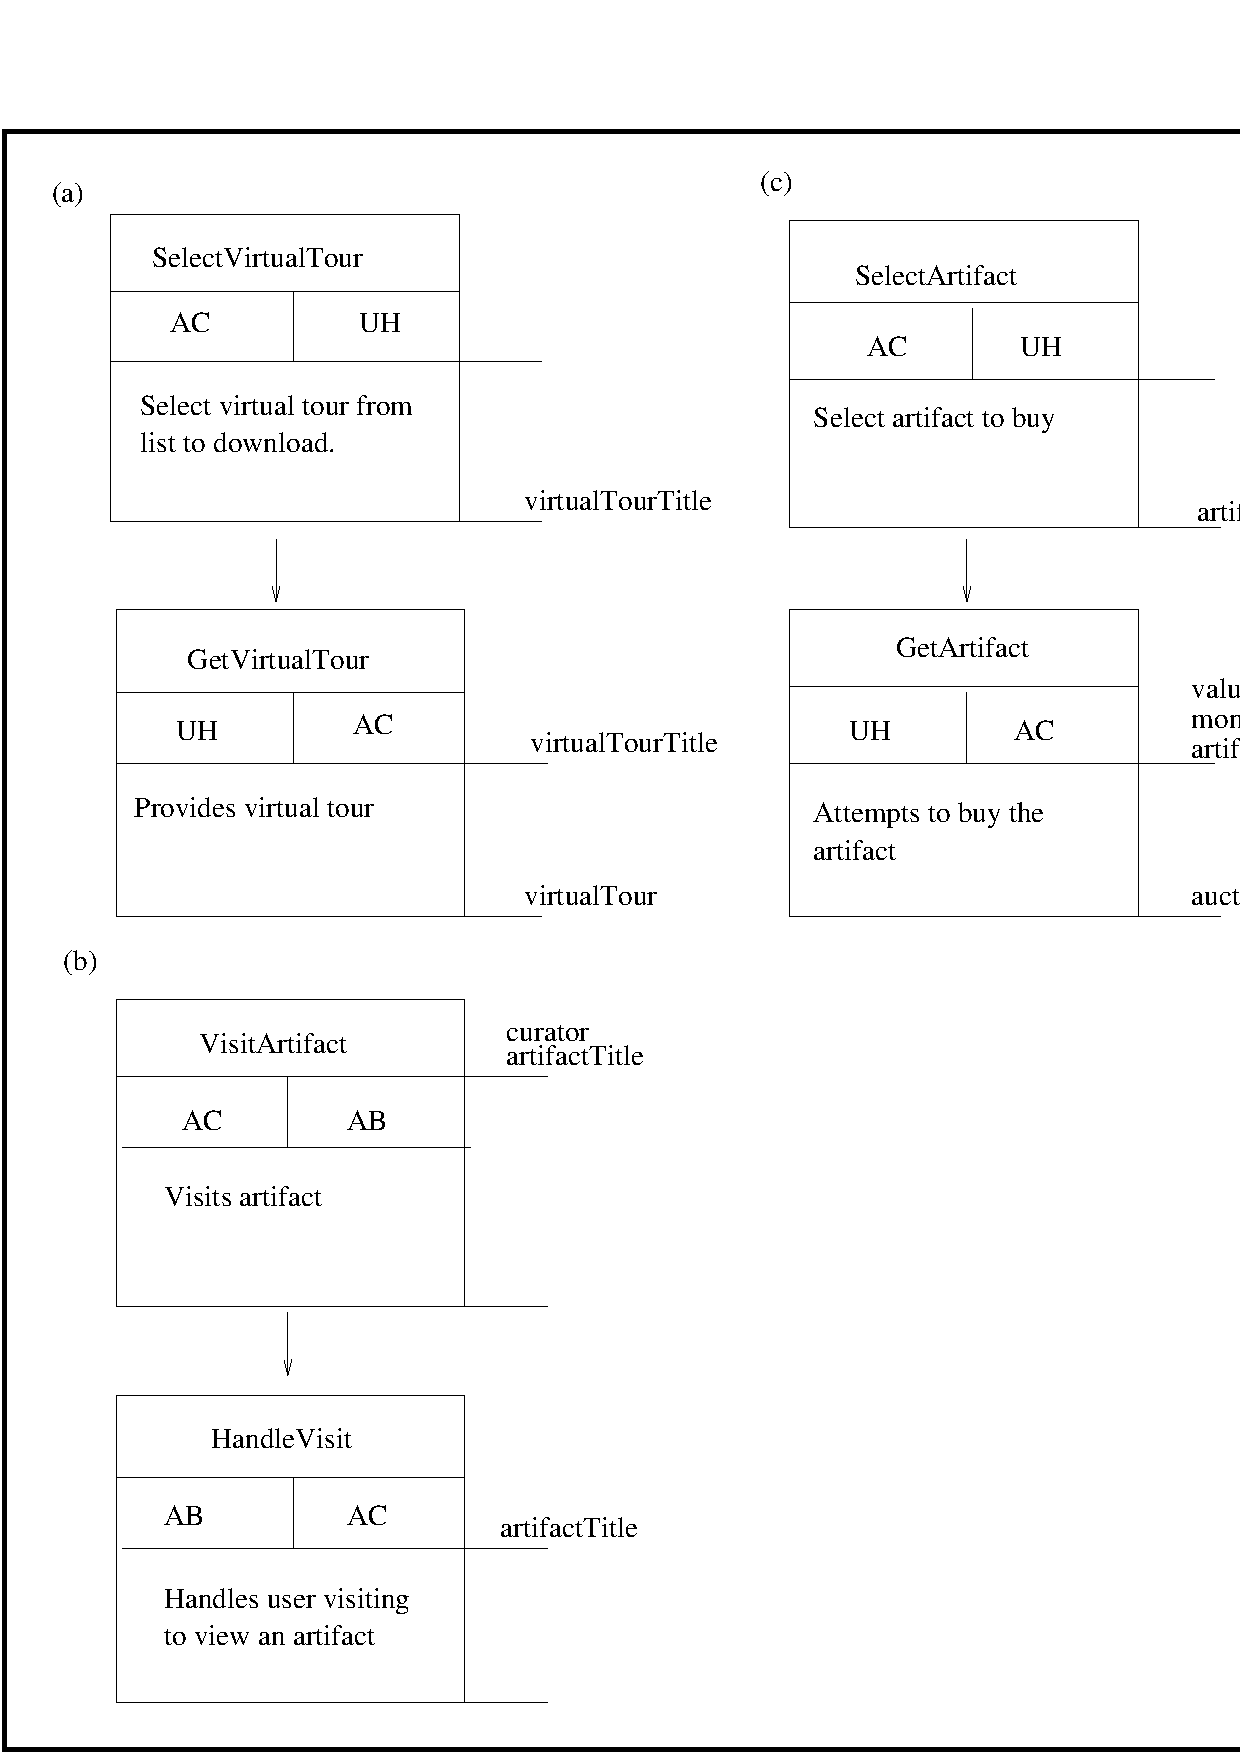
\includegraphics{ac_protocol.pdf}
    }
    \caption{Definition of protocols associated with the \textsc{ArtConsumer} role: (a) \fontfamily{\sfdefault}\selectfont DownloadVirtualTour, (b) BuyArt}
    \label{fig:ac_protocol}
  \end{center}
\end{figure}
\begin{figure}[H]
  \begin{center}
    \scalebox{0.70}{
      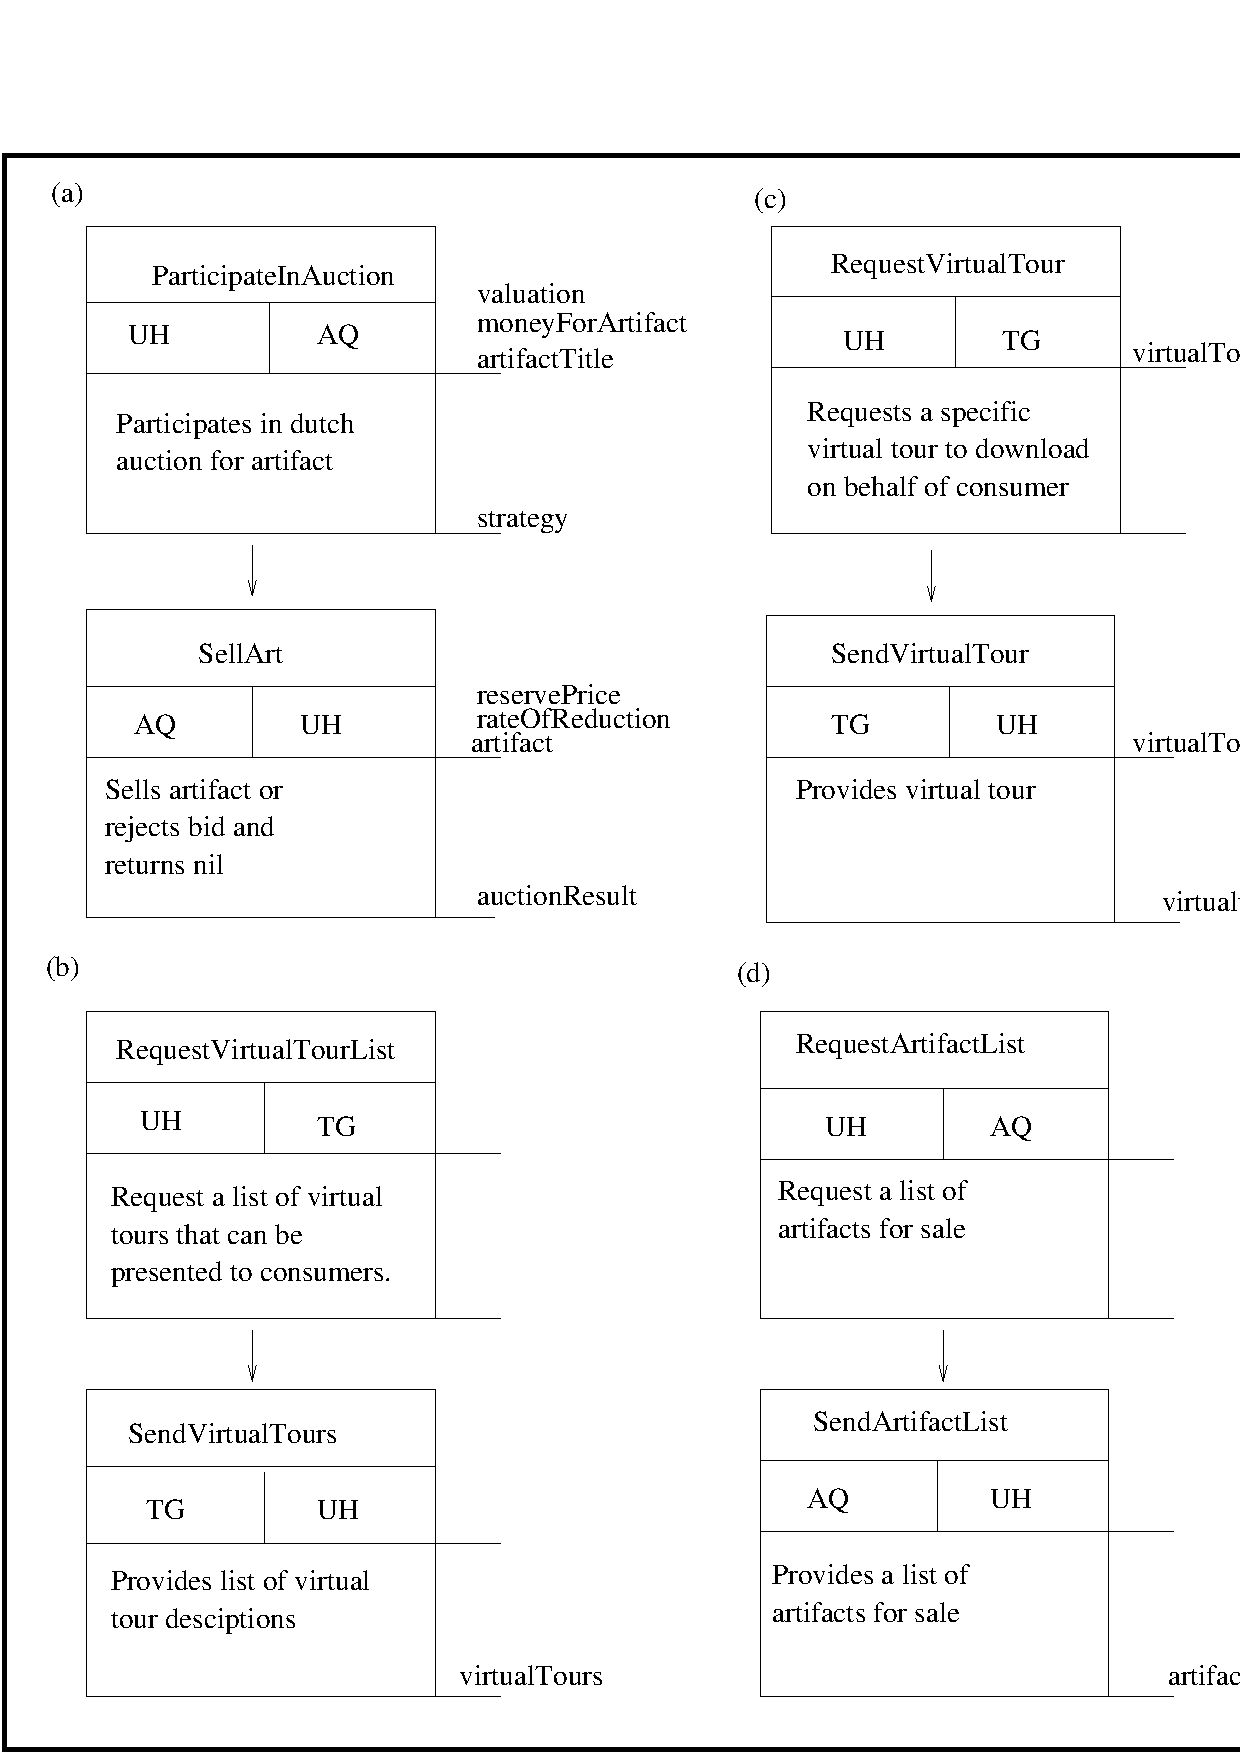
\includegraphics{uh_protocol.pdf}
    }
    \caption{Definition of protocols associated with the \textsc{UserHandler} role: (a) \fontfamily{\sfdefault}\selectfont ManageArtPayment, (b) GetVirtualTourList, (c) GetVirtualTour, (d) GetArtifactsList}
    \label{fig:uh_protocol}
  \end{center}
\end{figure}
\begin{figure}[H]
  \begin{center}
    \scalebox{0.70}{
      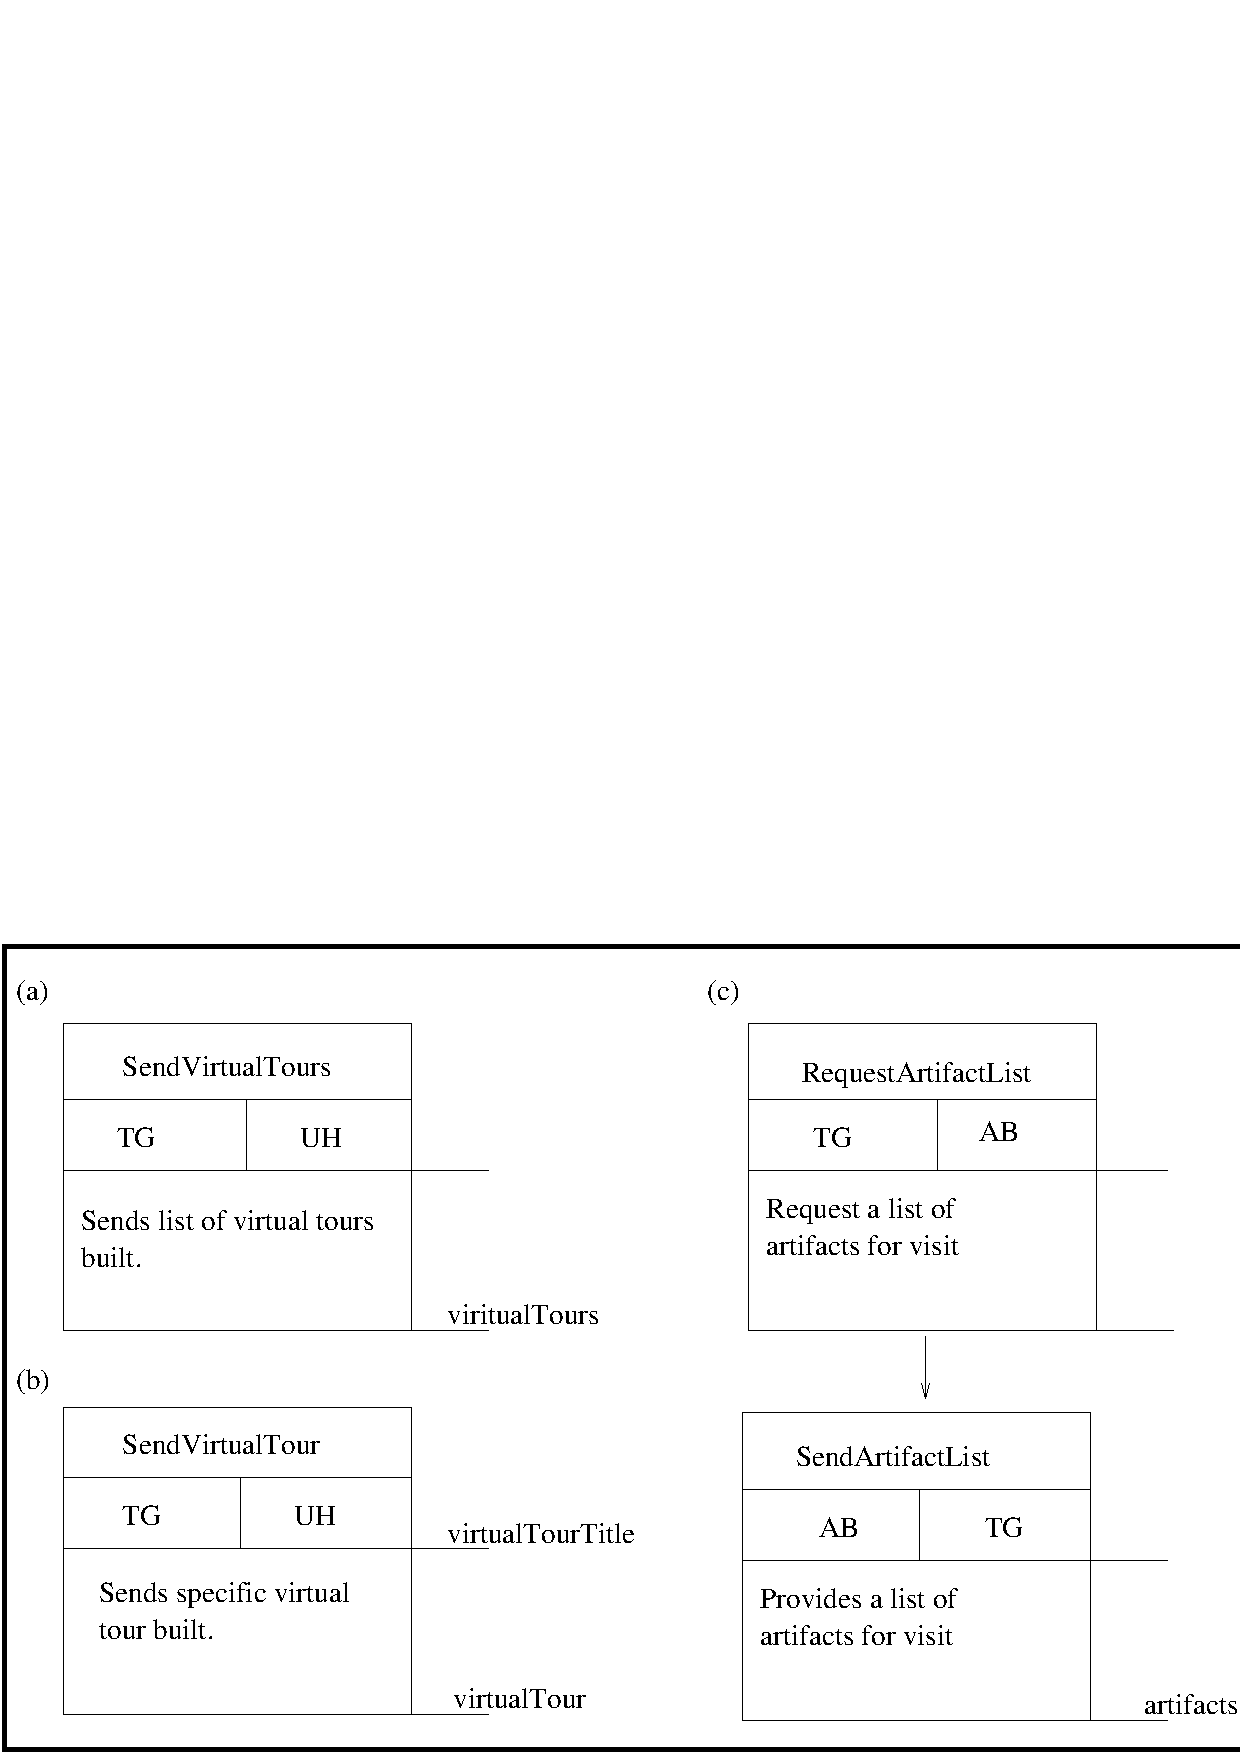
\includegraphics{tg_protocol.pdf}
    }
    \caption{Definition of protocols associated with the \textsc{TourGuide} role: (a) \fontfamily{\sfdefault}\selectfont SendVirtualTours, (b) SendVirtualTour, (c) GetArtifactList}
    \label{fig:tg_protocol}
  \end{center}
\end{figure}
\begin{figure}[H]
  \begin{center}
    \scalebox{0.70}{
      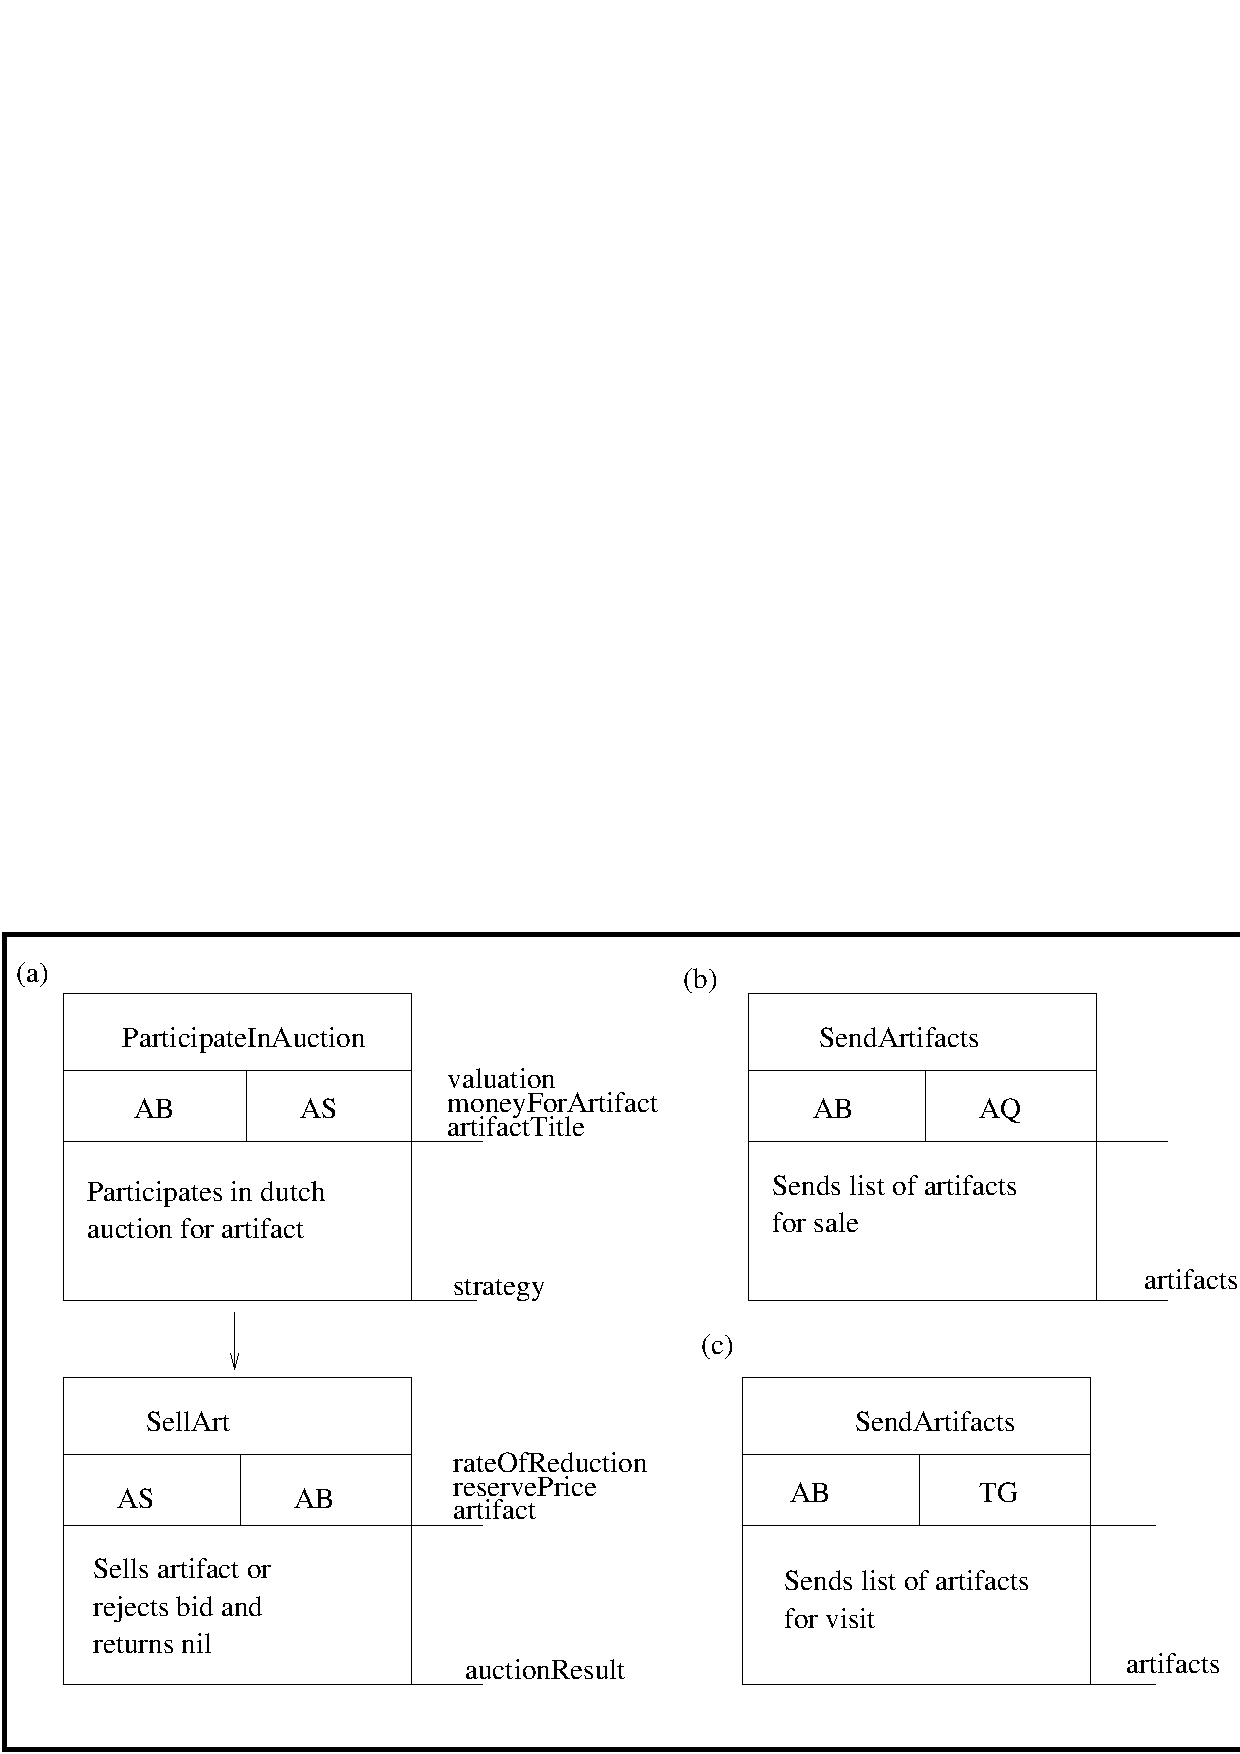
\includegraphics{ab_protocol.pdf}
    }
    \caption{Definition of protocols associated with the \textsc{ArtBuyer} role: (a) \fontfamily{\sfdefault}\selectfont BuyArt, (b) SendArtifacts}
    \label{fig:ab_protocol}
  \end{center}
\end{figure}

\begin{figure}[H]
  \begin{center}
    \scalebox{0.70}{
      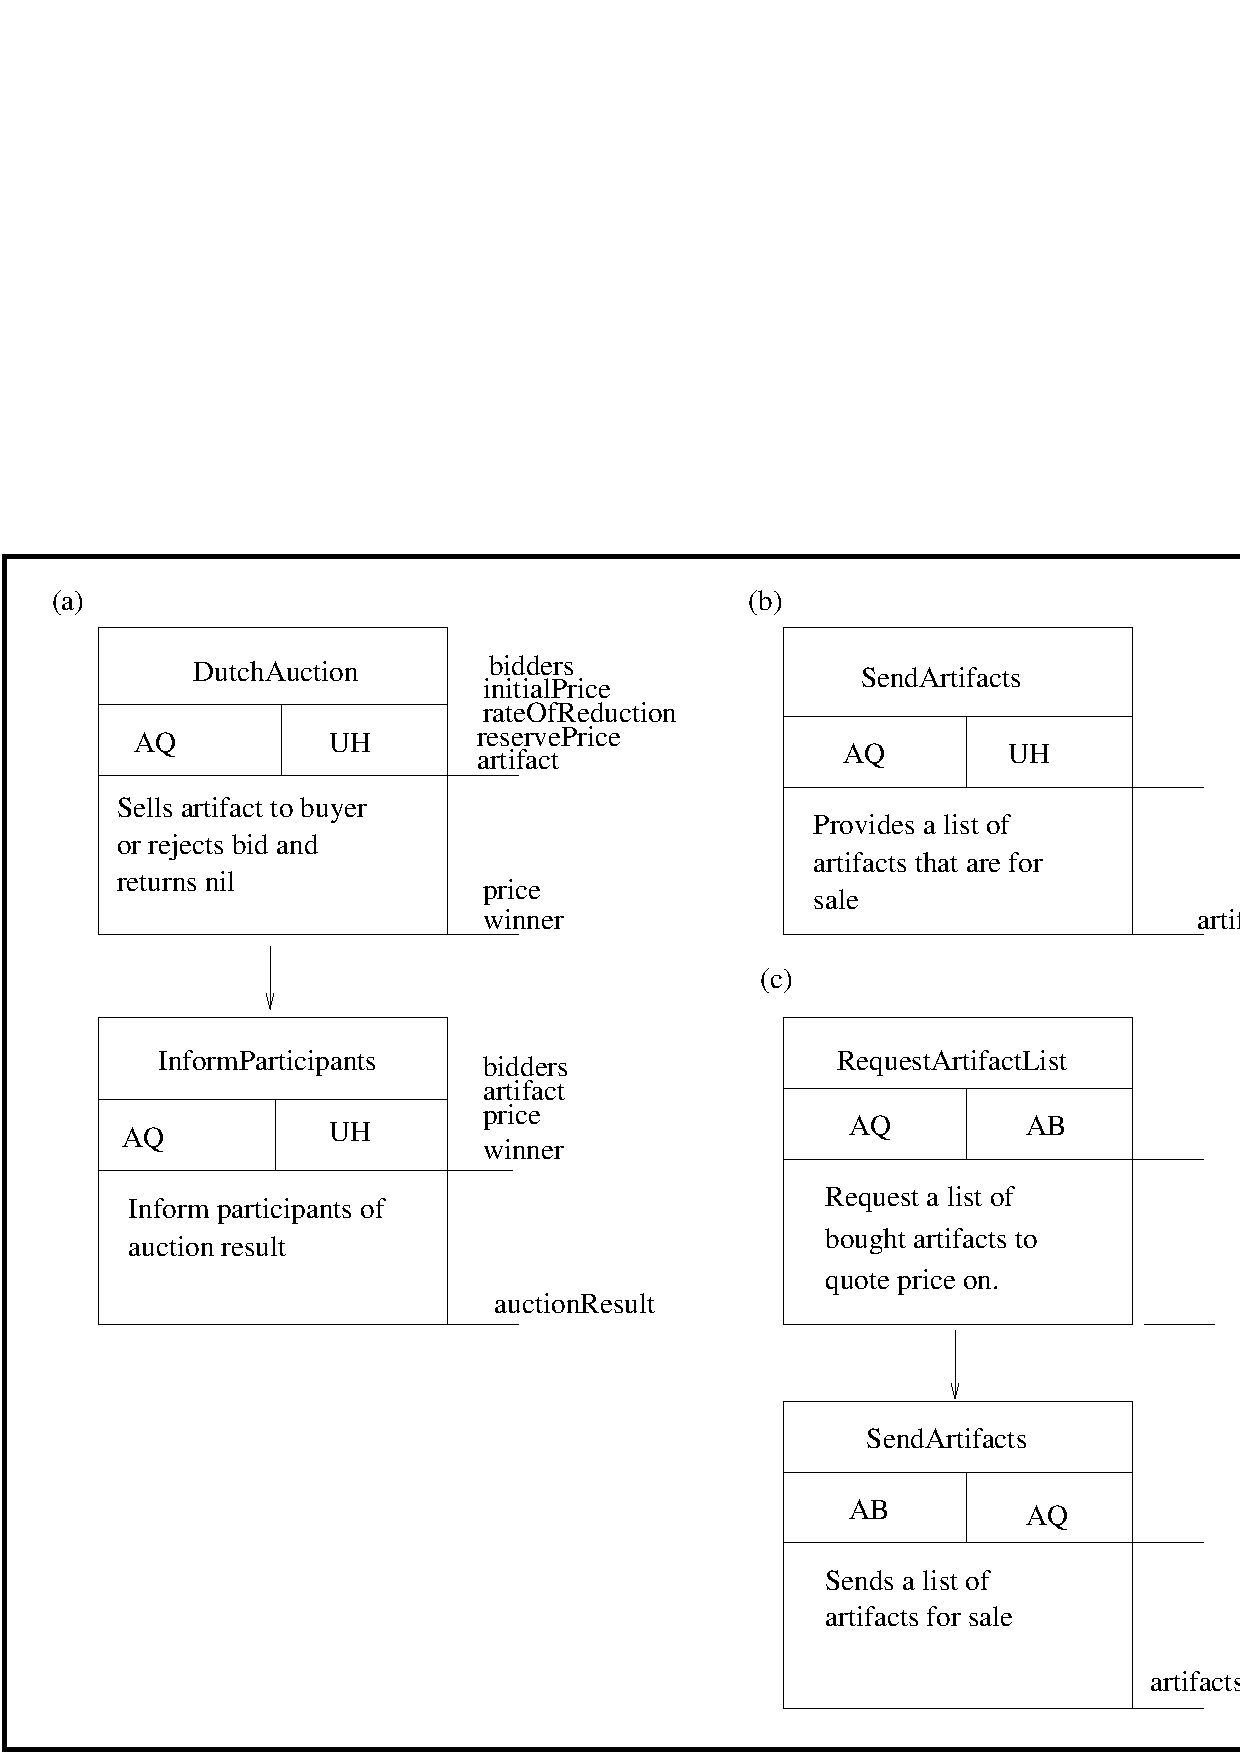
\includegraphics{aq_protocol.pdf}
    }
    \caption{Definition of protocols associated with the \textsc{ArtQuoter} role: \fontfamily{\sfdefault}\selectfont (a) SellArt, (b) GetArtifacts, (c) SendArtifacts}
    \label{fig:aq_protocol}
  \end{center}
\end{figure}
\begin{figure}[H]
  \begin{center}
    \scalebox{0.70}{
      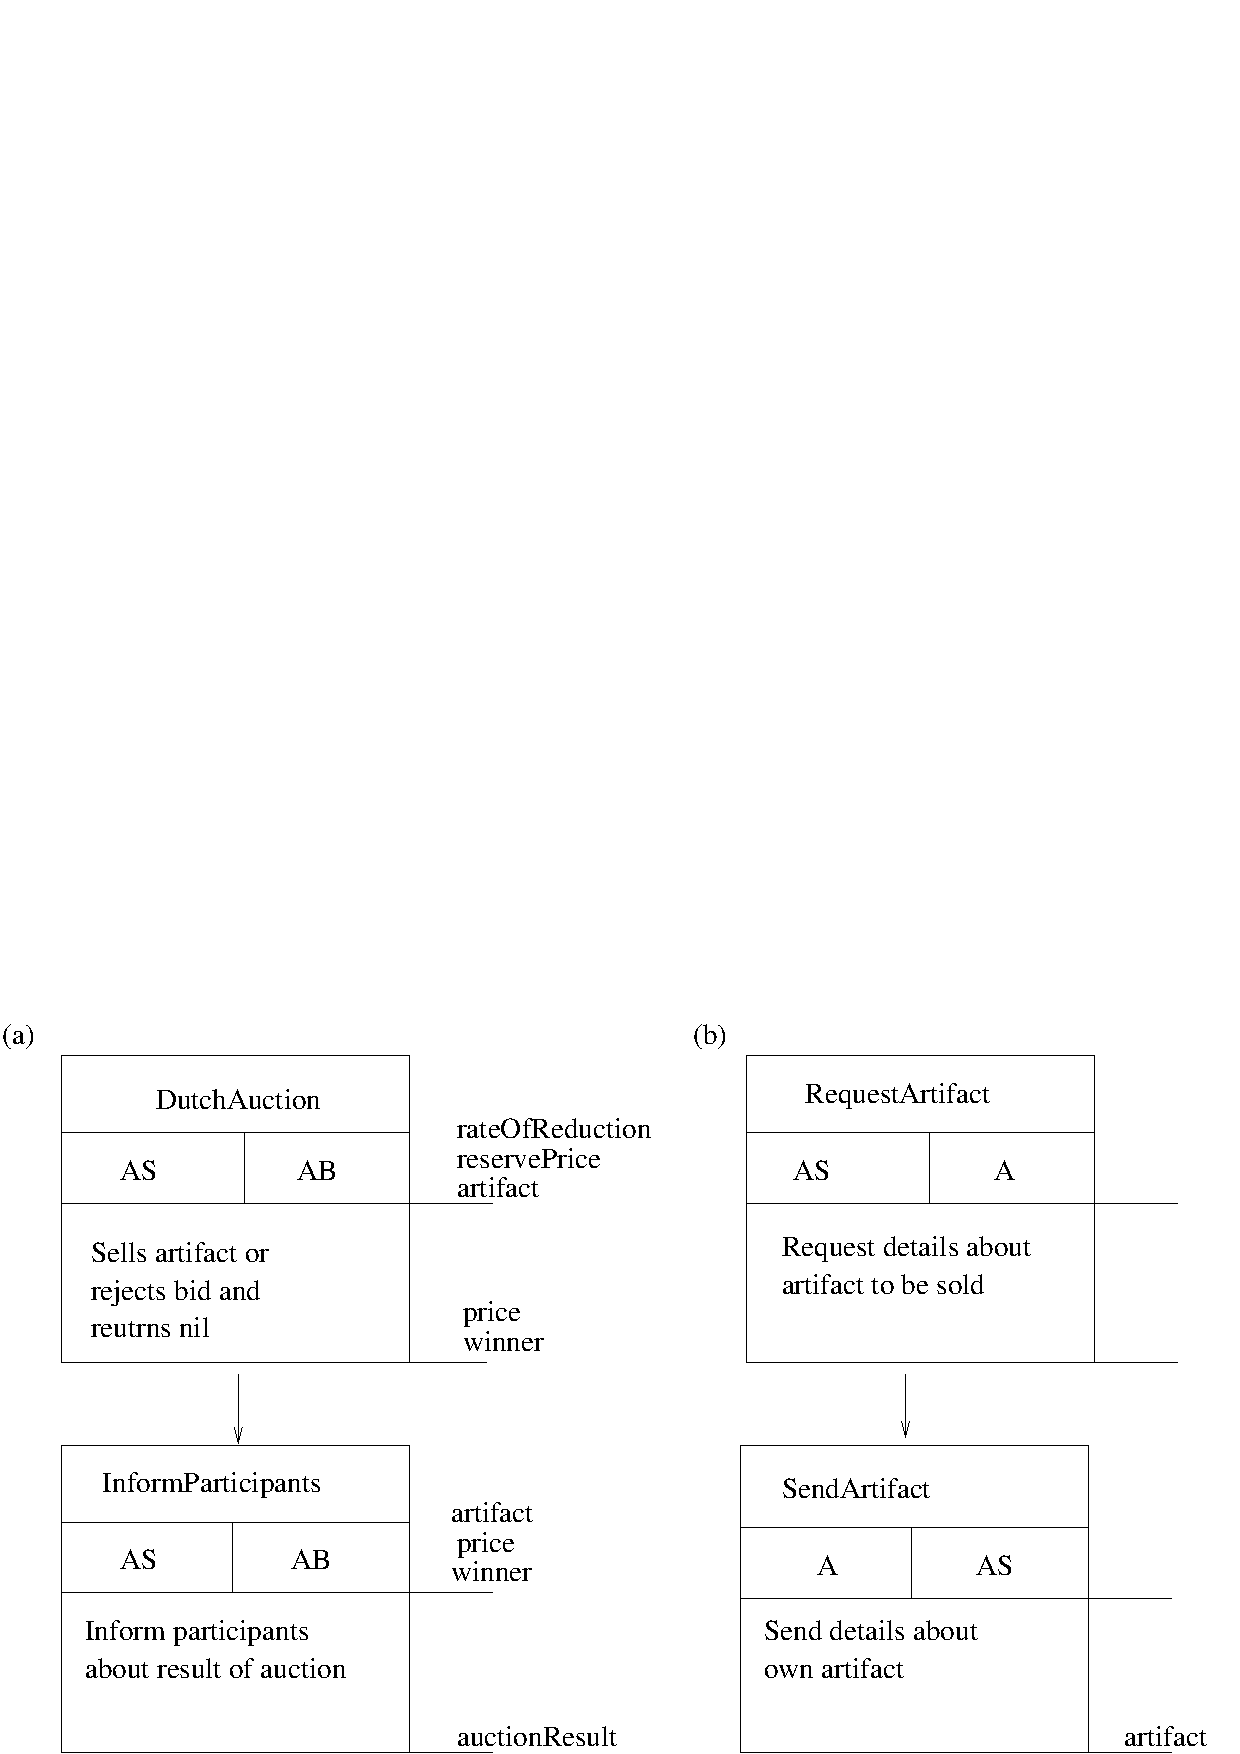
\includegraphics{as_protocol.pdf}
    }
    \caption{Definition of protocols associated with the \textsc{ArtSeller} role: \fontfamily{\sfdefault}\selectfont (a) SellArt, (b) GetArtDetails}
    \label{fig:as_protocol}
  \end{center}
\end{figure}
\begin{figure}[H]
  \begin{center}
    \scalebox{0.70}{
      \includegraphics{a_protocol.pdf}
    }
    \caption{Definition of protocols associated with the \textsc{Artist} role: \fontfamily{\sfdefault}\selectfont (a) SendArtDetails}
    \label{fig:a_protocol}
  \end{center}
\end{figure}
\subsection{Design}


\bibliography{references}{}
\bibliographystyle{plain}
\end{document}
